\chapter[Modelo de Caso de Uso]{Modelo de Caso de Uso}
Este documento apresenta o modelo de caso de uso, onde é desenvolvido um esquema e modelo básico das funções pretendidas do sistema e respectivamente os atuadores em seu ambiente. 

\section{Diagrama de Caso de Uso}
\begin{figure}[!h]
\centering
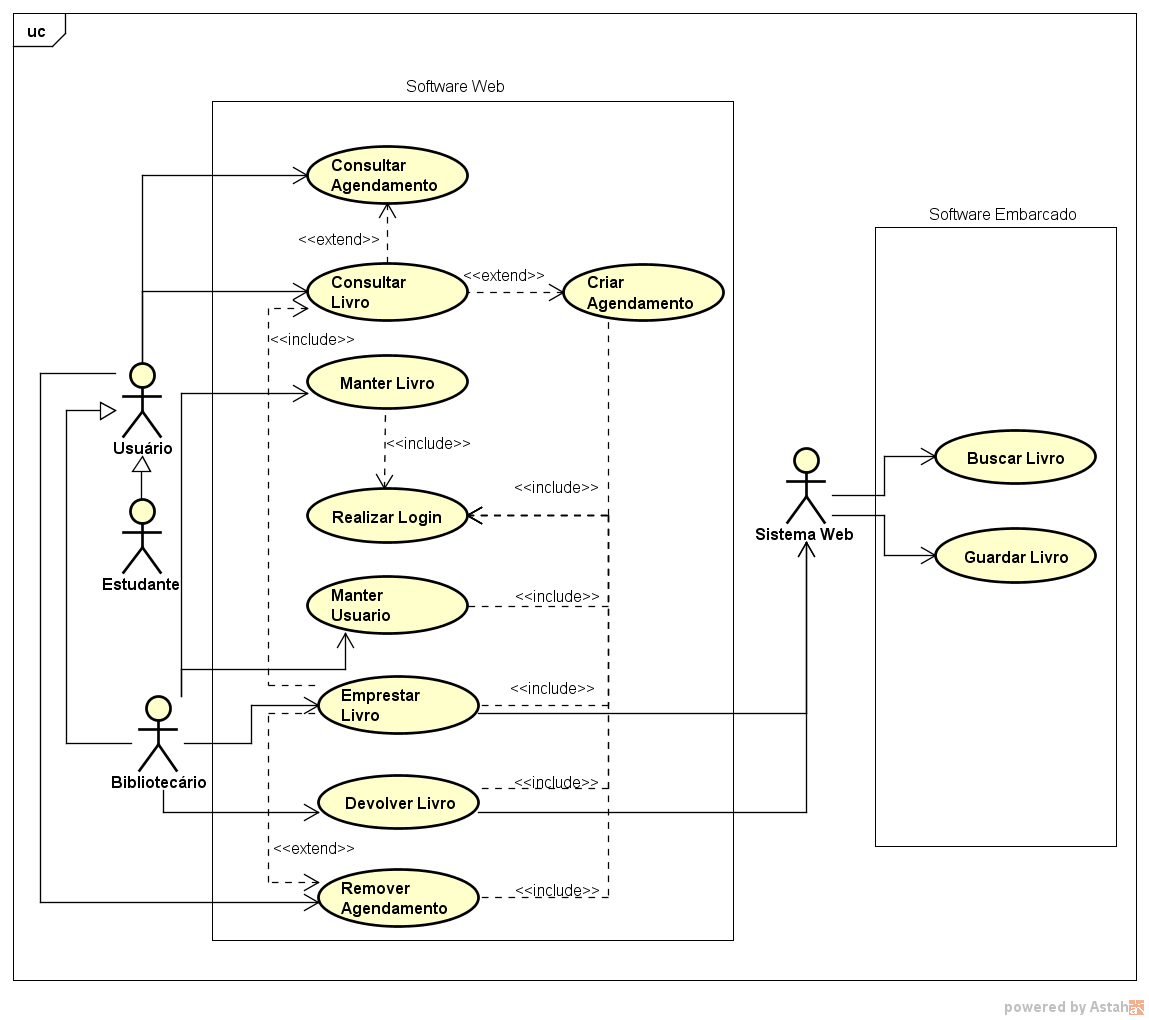
\includegraphics[scale=0.50, angle = 360]{figuras/caso_uso}
\caption[]{Diagrama de Caso de Uso para o projeto de software \textit{Bibliotech} (fonte: autor)
}
\end{figure}
\FloatBarrier

\section{Descrição de Casos de Uso}

\subsection{Consultar Agendamento}
Este caso de uso permite ao USUÁRIO consultar um agendamento realizado, e está consulta deve ser criada a partir do preenchimento de um formulário.

\subsection{Consultar Livro}
Este caso de uso permite ao USUÁRIO consultar a disponibilidade de um livro no sistema, e está consulta deve ser criada a partir do preenchimento de um formulário.

\subsection{Criar Agendamento}
Este caso de uso permite ao USUÁRIO criar um agendamento de solicitação de livro, e está consulta deve ser criada a partir do preenchimento de um formulário.

\subsection{Manter Livro}
Este caso de uso permite ao BIBLIOTECÁRIO cadastrar, alterar, remover e consultar informações de um livro no sistema.

\subsection{Realizar Login}
Este caso de uso permite ao BIBLIOTECÁRIO identificar-se para que eventuais permissões lhe sejam concedidas.

\subsection{Manter Usuário}
Este caso de uso permite ao BIBLIOTECÁRIO cadastrar, alterar, remover e consultar informações de um USUÁRIO.

\subsection{Emprestar Livro}
Este caso de uso permite ao BIBLIOTECÁRIO emprestar um livro a um USUÁRIO, e associar o empréstimo. Este empréstimo deve ser criado a partir do preenchimento de um formulário. 

\subsection{Devolver Livro}
Este caso de uso permite ao BIBLIOTECÁRIO devolver um livro e finalizar o empréstimo realizado a um USUÁRIO. 

\subsection{Remover Agendamento}
Este caso de uso permite ao BIBLIOTECÁRIO remover um agendamento de solicitação de livro,e está consulta deve ser criada a partir do preenchimento de um formulário.

\subsection{Buscar Livro}
Este caso de uso permite ao SISTEMA \textit{WEB} solicitar ao robô a busca física de um livro em seu respectivo endereço físico.

\subsection{Guardar Livro}
Este caso de uso permite ao SISTEMA \textit{WEB} solicitar ao robô devolução física de um livro em seu respectivo endereço físico.

